\chapter{Implementation}

\section{Implementation Overview}

The implementation begins by finding all eligible methods to be injected using the verification process indicated in Figure~\ref{logical_inclusion}. Each eligible method will have one or more aspects applied to it. The actual injection process will loop through each aspect for the eligible method and inject the necessary CIL instructions.

The CIL instructions modification is performed by using the open-source Mono.Cecil library. Originally, the System.Reflection APIs in the .NET Framework were favored, but it was later determined that Mono.Cecil provides more features and is much easier to work with. Buffalo uses Mono.Cecil heavily to modify CIL instructions and to assemble the final assembly.

\section{MethodBoundaryAspect Implementation Detail}

Each type of aspect has its own injector that implements the IInjectable interface. This interface contains only one method contract - Inject(..). It takes the list of eligible methods and injects the appropriate aspect to them.

MethodBoundaryAspect is pretty straightforward to implement. Take the following hello-world example wrapped in a try-catch-finally block as mentioned previously:

\begin{minipage}{\textwidth}
\begin{lstlisting}[caption={SayHello Function}, label=sayhello]
public void SayHello()
{
   try{
       Console.WriteLine(“Hello World!”);
   }catch(Exception ex){
   }finally{
   }
}
\end{lstlisting}
\end{minipage}

The generated CIL is shown in Figure~\ref{methodboundaryB4}. For ease of display, the CIL has been cleaned up a bit:

\begin{minipage}{\textwidth}
\begin{lstlisting}[caption={CIL Generated for Sample C\# Function}, label=methodboundaryB4]
.try
{
   .try
   {
      IL_0002: Ldstr "Hello World!"
      IL_0007: call void [mscorlib]System.Console::WriteLine(string)
      IL_000e: leave.s IL0015
   }
   catch [mscorlib]System.Exception
   {
      IL_0010: stloc.0
      IL_0013: leave.s IL_0015
   }
   IL_0015: leave.s IL_001c
}
finally
{
   IL_001a: endfinally
}
IL_001c: ret
\end{lstlisting}
\end{minipage}

Figure~\ref{methodboundaryB4} shows the standard emission of the CLR when it encounters the try-catch-finally statement. In CLR, there is a concept of the protected region, where each region is associated with a handler. A try-catch-finally is actually encapsulated in two such regions: a catch and a finally. From here, it can be easily figured out where to inject the various boundary aspects, as shown in Figure~\ref{methodboundary02}.

\begin{figure}[H]
  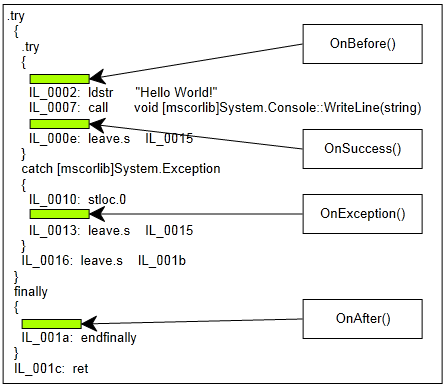
\includegraphics[scale=1.0]{MethodBoundaryOverview.PNG}
  \centering
  \caption{CIL Interception Points\label{methodboundary02}}
\end{figure}

\section{MethodAroundAspect Implementation Detail}

The MethodAroundAspect, on the other hand, is a much more complicated when compared to the MethodBoundaryAspect.

MethodAroundAspect implements IMethodAroundAspect which has the following contract:

\begin{minipage}{\textwidth}
\begin{lstlisting}[caption={IMethodAroundAspect Interface}, label=aroundcontract]
internal interface IMethodAroundAspect : IAspect
{
	void Invoke(MethodArgs args)
}
\end{lstlisting}
\end{minipage}

In the development of an aspect, a Proceed() can be issued to signal a call back into the original method. The steps taken to implement MethodAroundAspect in CIL are roughly as follows:

\begin{enumerate}
	\item Create a replacement for the annotated function with exactly the same method signature.
	\item Create and store a variable pointing to the aspect.
	\item Copy all parameters from original method to the newly created replacement function.
	\item Create a variable to hold MethodArgs.
	\item Issue a call to Invoke() from the replacement function, passing in the MethodArgs variable.
	\item Handle the return value appropriately.
	\begin{enumerate}
		\item If the original method returns non-void type, then put the return value back on the stack.
		\item If the original method returns void, discard the return value from Invoke().
	\end{enumerate}
	\item Handle Proceed() that might be issued from inside the Invoke().
	\begin{enumerate}
		\item Load all the parameters onto the stack.
		\item Call back into the original method.
		\item Handle the return value appropriately.
	\end{enumerate}
	\item Modify all calls from original method to the replacement method.
\end{enumerate}

As Figure~\ref{around_overview} shows, the actual calling of either the original or replacement method is abstracted away. This is also a testament of the saying in software engineering that "anything can be resolved by another layer of abstraction."

Another important distinction is that MethodAroundAspect currently can be applied only on the method level, and that it should be applied to one method only. This is by design because a replacement method might not be appropriate to replace more than one method. Especially if the aspect is applied on the assembly level, all the public methods will be replaced by a single replacement method.

\section{MethodArgs Implementation Detail}

When an aspect is being developed, information about the target method can be accessed. This is achieved by using the MethodArgs object. During the weaving, an instance of MethodArgs is created with all properties assembled dynamically to capture the information of the current executing method. This instance of MethodArgs is then passed as a parameter into each of the joint points of the aspect.

Being able to capture some information about the annotated methods will be  extremely useful in cases where debugging becomes necessary.

A distinct instance of MethodArgs for each boundary aspect was instantiated in an early Buffalo implementation. Later on as an optimization, only one instance is instantiated at the beginning of the method body, and that instance is used in all the boundary aspects for a target method.

An example of how to use MethodArgs is presented in the user manual.
